\section{Methodology}


\subsection{Overview}
\label{sec:LEOMDL}

Satellites are assumed to be geometry awareness, i.e., knowledge of the topology and geometry and dynamics of the network are available to satellites. Satellites, even in small satellites with limited processing capacity, are geometry awareness because Attitude and Determination and Control subsystem (ADCS), which is used to point to neighbor satellites for intersatellite communication, shall rely on geometry awareness.

We adopt hop-by-hop shortest path routing based on Manhattan distance. Every node has two neighbors on the shortest path to the destination, except for the source node and the destination node are on the same orbit or same row, there may not exist two neighbors on the shortest path to the destination. In that case, we only choose the shortest one to avoid route oscillation.

Before a transmission, every node chooses one of the two neighbors according to the status that includes the remaining power, congestion level, and the instability of ISL.

The cost when a local satellite chooses a neighbor satellite $S_n$ as its next hop can be calculated as below.

\begin{equation}
	Cost_{n}=C_{n}+k \cdot P_{n}+I_{n}
\end{equation}
where $C_n$ is the congestion level of satellite $S_n$, $P_n$ is the power burden of satellite $S_n$ and $I_n$ is the instability of $S_n$.
Weighting factor $k=1-\frac{MD(S_n,\ D)}{d}$ blongs to $[0,1]$,  where $MD(S_n,\ D)$ is the Manhattan distance between satellite $S_n$ and the destination satellite, and $d$ is the diameter of the network (which is a constant). The times of splitting flow increases with distance, so  $k$, which represents the significance of energy, should increase hop-by-hop. Then $Cost_1$ and $Cost_2$ are the costs of the two neighbors, $S_1$ and $S_2$ repectively. The probability of sending a packet to $S_1$ is $\frac{Cost_2}{Cost_1+Cost_2}$ and to $S_2$ is $\frac{Cost_1}{Cost_1+Cost_2}$.


\subsection{ISL Instability}
Owing to the physical limits of the antenna, the link stability between two  satellites depends on their relative distance and velocity \cite{ISL1}\cite{ISL2}.
Intra-plane ISLs are stable because the distance is nearly constant but inter-plane ISLs are unstable because the distance and the relative velocity change with latitude. Clearly, the distance of inter-plane ISL is: 

\begin{equation}
 \operatorname{dist}\left(l a t^{\circ}\right)=r \sqrt{2} \cos \left(l a t^{\circ}\right) \cdot \sqrt{1-\cos \left(360^{\circ} \frac{1}{2 w}\right)} 
 \label{eq:INTERISL}
\end{equation}

where $r$ is the radius of the plane, $lat^{\circ}$ stands for the latitude at which the center of the ISL resides, and $w$ is the number of orbits.

And we define the function of normalizing instability of inter-plane ISL is:
\begin{equation}
 I\left(l a t^{\circ}\right)=\frac{\operatorname{dist}\left(l a t^{\circ}\right)-\operatorname{dist}\left(66.34^{\circ}\right)}{\operatorname{dist}\left(0^{\circ}\right)-\operatorname{dist}\left(66.34^{\circ}\right)} \cdot M A X^{\lambda} 
 \label{eq:NORMALIZEDINSTABILITY}
\end{equation}

\begin{equation}
 \lambda=\left\{\begin{array}{ll}1, & \text { opposite direction / in polar region } \\ 0, & \text { same direction }\end{array}\right. 
\end{equation}

where $\lambda \in \{0,1\}$, if $\lambda = 1$ , it represents the two satellites move in the opposite directions or one of the satellites is in the polar region. if $\lambda = 0$, it means that two satellites move in the same direction and both of them are not in the polar region, and $MAX$ is an extremely large number.

Then the instability $I_n$ of local satellite ISL to satellite $S_n$ is defined as follows. 
\begin{equation}
 I_{n}=\left\{\begin{array}{ll}I\left(l a t_{n}^{\circ}\right), & \text { inter-plane ISL } \\ 0, & \text { intra-plane ISL }\end{array}\right. 
 \label{eq:INSTABILITY}
\end{equation}

Notice that the intra-plane ISL is stable, so $I_n$ always equals 0 on intra-plane ISL.

\subsection{Energy Burden of Satellite}
\subsubsection{Energy level of satellite}
Although neighboring satellites could acquire the status of each other by the "Hello message" \cite{OPSPF},  frequently exchanging hello message is still bandwidth consuming and  may make the congestion on links more severe. Hence, we make use of the satellite historical position information to estimate the remaining energy.

During eclipse time, when satellites pass through a shadow region on the opposite side of the earth from the sun, satellites are powered by batteries. The longer time a satellite in the eclipse area (the shadow of the Earth), the more power of satellite's battery is consumed. There are two common ways to acquire satellite energy information: First, every satellite will flood its energy status to the whole network periodically. Second, the satellite will tell the ground station or GEO satellites their energy status, then other satellites can obtain the energy status through the ground station or the GEO satellites. 

Although state of health (e.g, energy level information) of satellites are usually periodically transmitted to ground server or GEO, due to limit density of ground server and bandwidth consumption,  energy level information (e.g., state of charge) of other satellites are not available.  To prolong of satellite life time, energy level of neighboring statellites are also considered in our scheme. 

We use TLE of neighboring satellites to estimate their remaining energy level. 
In Figure \ref{fig:ELLIPSE}, the projection of the Earth’s shadow on the orbital plane of an satellite is an ellipse. Refer to \cite{ELLIPSE}, the semi-minor axis $b$ and semi-major axis $a$ of the ellipse are denoted as $b=R$ and $a=R\ csc\ i$, respectively, where $R$ is the radius of the earth and $i$ defines the inclination of the Sun onto the orbital plane of the satellite. The equation of an ellipse is given by 

\begin{equation}
 \delta^{2}=\frac{b^{2}}{1-e^{2}(\cos \theta)^{2}} 
 \label{eq:ELLIPSE}
\end{equation}
where $\delta$ is the distance from the center to either vertex of the ellipse, and $\theta = \angle SOC$, measured in the orbit plane between the satellite $S$ and the conjunction point $C$ (the intersection of the satellite orbit and the straight line between the Earth and Sun).

The eccentricity of an ellipse is given by
\begin{equation}
 e=\frac{\sqrt{a^{2}-b^{2}}}{a}
 \label{eq:ECCENTRICITY}
\end{equation}

\begin{figure}[H]
	\centering
	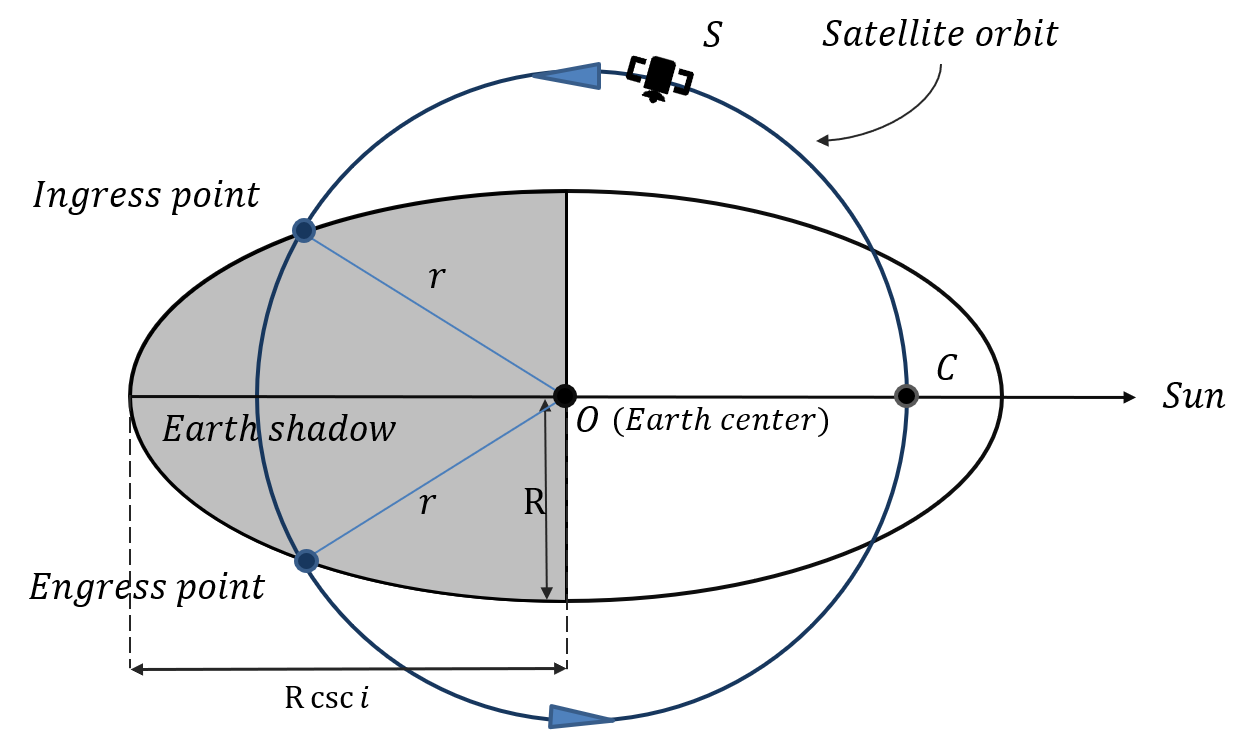
\includegraphics[scale=0.9,clip, width=0.4\textwidth]{fig/ellipse.png}	
	\caption{The shadow area, the angle of ingress/egress.}
	\label{fig:ELLIPSE}
\end{figure}

Substituting $a=R\ csc\ i$ and $b=R$ into eq(eccentricity). After little reduction, yields 

\begin{equation}
 e=\cos i 
\end{equation}

The ingress/egress point is when the distance between a point on the ellipse edge and the ellipse center equals the radius of the satellite orbit $r$.
Then the equation  \ref{eq:ELLIPSE} can be written as:
\begin{equation}
 \delta_{i n}^{2}=r^{2}=\frac{R^{2}}{1-(\cos i)^{2}\left(\cos \theta_{i n}\right)^{2}} 
\end{equation}

where $\delta^2_{in}$ is the distance between the ingress and the center of earth, and $\theta_{in}$ is the angle when the satellite enters the shadow. Clearly, we have

\begin{equation}
 \cos \theta_{i n}=\pm \sqrt{\frac{1-\left(\frac{R}{r^{2}}\right)^{2}}{\cos i}} 
\end{equation}

The duration angle of a circular orbit satellite in the eclipse is $\theta_E$, denoted as
\begin{equation}
 \theta_{E}=2\left(180^{\circ}-\theta_{i n}\right) 
 \label{eq:DURATONANGLE}
\end{equation}

Now the shadow interval can be obtained from
\begin{equation}
 t_{S H}=\frac{\theta_{E}}{360^{\circ}} \cdot P 
 \label{eq:SHADOWINTERVAL}
\end{equation}
where $P$ is the period of the satellite.

We set the $\theta = 0^{\circ}$ as the start of a period,**then the time of a satellite entering the eclipse is 
\begin{equation}
 t_{\text {enter }}=\frac{\theta_{\text {in }}}{360^{\circ}} P 
 \label{eq:ENTERINGTIME}
\end{equation}

Let $S_{n,t_{d}}^{\text {energy }}$ represent the total energy consumption of satellite $S_n$ in the $t_{d}$ time.
\begin{equation}
 T_{d}=t_{\text {current }}-t_{\text {enter }} 
\end{equation}

where $t_{current}$ is the current time.

In every time slot, satellite $S_n$ will obtain a traffic density level mapped to the ground. In this work, we viewed the traffic density level as the power consumption since the traffic density is significantly positively correlated with the power consumption. Thus the estimated power consumption of satellite $S_n$ can be the sum of the traffic density level in the $t_{d}$ time:
\begin{equation}
 S_{n, t_{d}}^{\text {energy }}=\sum_{t=t_{e n t e r}}^{t_{d}} D_{n}^{t} 
\label{eq:ENERGYCONSUMPTION}
\end{equation}

where $D_n^t$ is the density level of satellite $S_n$ at time $t$.
Then we normalized the power consumption to
\begin{equation}
  \frac{S_{n, t_{d}}^{\text {energy }}-\min S_{n,t_{d}}^{\text {energy }}}{maxS_{n,t_{d}}^{\text {energy }}-\min S_{n,t_{d}}^{\text {energy }}}
\label{eq:ENERGYCONSUMPTION}
\end{equation}

\subsubsection{Orbit Section}
Except for estimating the power consumption of satellites, we take a step further by classifying the energy burden of using a satellite in different sections of an orbit.
We divide an orbit into 4 sections:

\begin{itemize}
  \item Sunlight section
  \item Just entered the eclipse section
  \item Middle of the eclipse section
  \item About to leave the eclipse section
\end{itemize}

\paragraph{Sunlight section}
In the sunlight section, the satellite is powered by sunlight, and the battery is also being charged, so the remaining energy of battery is sufficient.

\paragraph{Just entered the eclipse section}
The satellite is powered by a battery but the satellite just entered the eclipse area, so the remaining battery power is regarded as sufficient as well.
\begin{equation}
  if\  \frac{t_{\theta_{n}}-t_{\text {enter }}}{t_{S H}}<\frac{1}{3} \rightarrow  just\ entered\ the\ eclipse\ section
\end{equation}

where $t\theta_n$ is the angle of satellite $n$ of current time,  $t_{\theta_n}-t_{enter}$ can be represented how long has a satellite been in the eclipse time.

\paragraph{Middle of the eclipse section}
The satellite is powered by a battery, and the satellite has already entered the eclipse area for a while; thus, the remaining battery power is relatively viewed as less.
\begin{equation}
  if\  \frac{t_{\theta n}-t_{\text {enter }}}{t_{S H}}<\frac{2}{3} \rightarrow  middle\ of\ the\ eclipse\ section
\end{equation}

\paragraph{About to leave the eclipse section}
The satellite is powered by a battery, and the satellite has already entered the eclipse area for a long time; thus, the remaining battery power is less than the satellite in the middle of the eclipse zone. In this paper, we focus on the DoD of the battery issue, so we should not view the satellite in this zone as a proper next hop.
\begin{equation}
  if\  \frac{t_{\theta_{n}}-t_{\text {enter }}}{t_{S H}}<1 \rightarrow  about\ to\ leave\ the\ eclipse\ section
\end{equation}

After we divide the area of the eclipse, the concept of remaining energy can be transformed into the burden of using per satellite.
Every section is assigned to a burden factor $\gamma$ between 0 and 1. The satellite's power burden is positively correlated with the burden factor. For example, when a satellite is in the sunlight section, which will not consume the battery power, its burden factor is 0. The expression and the burden factor of each section is shown in \ref{table:SECTION}.

\begin{table*}[h]
	\caption{Burden factor of section and the expression}
	\label{table:SECTION}
\begin{center}
\begin{tabular}{|l|l|l|}
\hline
\textbf{Section} & \textbf{Expression}      &  \textbf{Burden factor($\gamma$)}          \\  \hline
Sunlight section           			  & $ \cos \theta_{n}>\sqrt{\frac{1-\left(\frac{q}{q_{S H}}\right)^{2}}{\cos i}} $ or $ \cos \theta_{n}<-\sqrt{\frac{1-\left(\frac{q}{q_{S H}}\right)^{2}}{\cos i}} $  & 0.0  	\\ \hline
Just entered the eclipse section                   & $ \frac{t_{\theta n}-t_{\text {enter }}}{t_{S H}}<\frac{1}{3} $          													      &0.25	 \\ \hline
Middle of the eclipse section                      & $ \frac{1}{3}<\frac{t_{\theta n}-t_{e n t e r}}{t_{S H}}<\frac{2}{3} $               											      &0.5	\\ \hline
About to leave the eclipse section              & $ \frac{2}{3}<\frac{t_{\theta n}-t_{\text {enter }}}{t_{S H}}<1 $             												      &0.75	 \\ \hline

\end{tabular}
\end{center}
\end{table*}

Therefore, if we want to use satellite $S_n$ as the next hop, we not only have to consider its remaining energy but its current zone of eclipse. 
Here we define the potential energy risk as the probability of a satellite runs out of battery. We quntify the potential energy risk of Satellite $S_n$ is:
\begin{equation}
 P_{n}=\left(\frac{S_{n, t_{d}}^{\text {energy }}-\min S_{n, t_{d}}^{\text {energy }}}{\max S_{n, t_{d}}^{\text {energy }}-\min S_{n, t_{d}}^{\text {energ }}}\right) \cdot \gamma_{n},
\label{eq:POTENTIALENERGYRISK}
\end{equation}

where $\gamma_n$ is the burden factor of satellite $S_n$.
With the rise of the potential energy risk, a battery gets easier to become a high-DoD battery which will lead to a shorter life time.


\subsection{Congestion Level}
To estimate congestion level of satellites, we use the Discounting Rate Estimator (DRE) \cite{CONGA} , 
which is  similar to calculating an exponential moving average but is easier to implement,  and reacts faster to traffic bursts. 
In table[c], each satellite maintains a register, $V_n$ for each neighboring satellite $V_n$. 
$V_n$ is incremented for each packet sent to $V_n$  and is decremented periodically (every $T_{dre}$) with a multiplicative factor $\alpha$ between $0$ and $1$. More precisely,
\begin{equation}
 V_{n} \leftarrow V_{n} \times(1-\alpha) 
\label{eq:CONGA}
\end{equation}

So $V_n$ is proportional to the rate of traffic over the link to $S_n$. If the traffic rate is $Q_n$, then $V_n\approx Q_n \cdot \tau$, where $\tau = \frac{T_{dre}}{\alpha}$. The round trip time(RTT) of satellites is in 30ms to 50ms \cite{TELESAT}, and $T_{dre}$ could be a little larger than the RTT time.

Then the congestion level of neighboring satellite $S_n$ is calculated as:
\begin{equation}
 C_{n}=\frac{2 \cdot a \tan \left(V_{n} \cdot D_{n}\right)}{\pi} ,
\end{equation}

where $C_n$ is between $0$ and $1$, and $D_n$ is the density level of satellite $S_n$.



